% TikZ flowchart: a multi-step process with a loop
\documentclass{article}
\usepackage{tikz}
\usetikzlibrary{shapes.geometric, positioning, arrows.meta, fit, backgrounds}

\tikzset{
  startstop/.style={ellipse, draw=green!60!black, fill=green!10, thick,
    minimum width=2.5cm, minimum height=0.9cm, text centered, font=\small},
  process/.style  ={rectangle, draw=blue!60!black, fill=blue!8, thick,
    minimum width=3.5cm, minimum height=0.9cm,
    text centered, rounded corners=3pt, font=\small},
  decision/.style ={diamond, draw=orange!70!black, fill=orange!10, thick,
    aspect=2.5, minimum width=3.5cm, minimum height=0.9cm,
    text centered, font=\small},
  io/.style       ={trapezium, draw=purple!60, fill=purple!8, thick,
    trapezium left angle=75, trapezium right angle=105,
    minimum width=3cm, minimum height=0.9cm,
    text centered, font=\small},
  arrow/.style={thick, -{Stealth[length=6pt]}},
}

\begin{document}
\begin{figure}[h]
\centering
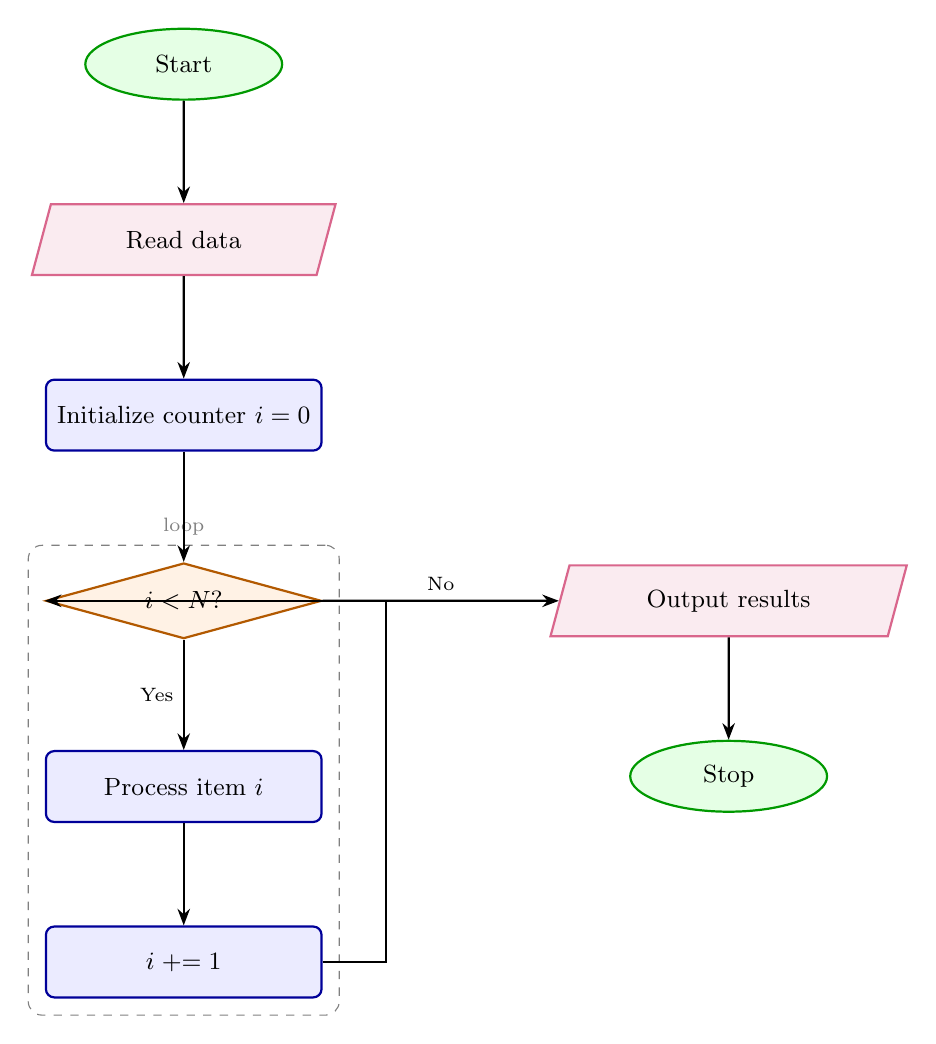
\begin{tikzpicture}[node distance=1.3cm]

  \node[startstop]                   (start)  {Start};
  \node[io,      below=of start]     (input)  {Read data};
  \node[process, below=of input]     (init)   {Initialize counter $i=0$};
  \node[decision,below=1.4cm of init](loop)   {$i < N$?};
  \node[process, below=1.4cm of loop](body)   {Process item $i$};
  \node[process, below=of body]      (inc)    {$i \mathrel{+}= 1$};
  \node[io,      right=3cm of loop]  (output) {Output results};
  \node[startstop,below=of output]   (stop)   {Stop};

  \draw[arrow] (start)  -- (input);
  \draw[arrow] (input)  -- (init);
  \draw[arrow] (init)   -- (loop);
  \draw[arrow] (loop)   -- node[left,  font=\scriptsize]{Yes} (body);
  \draw[arrow] (body)   -- (inc);
  % Loop back: go right, then up past loop, then back into loop from left
  \draw[arrow] (inc.east) -- ++(0.8,0) |- (loop.west);
  \draw[arrow] (loop.east) -- node[above, font=\scriptsize]{No} (output);
  \draw[arrow] (output) -- (stop);

  % Dashed box around the loop body
  \begin{scope}[on background layer]
    \node[fit=(loop)(body)(inc), draw=gray, dashed, rounded corners=5pt,
          inner sep=6pt, label={[font=\scriptsize, gray]above:loop}] {};
  \end{scope}

\end{tikzpicture}
\caption{Flowchart with loop and grouped region.}
\end{figure}
\end{document}
